\newpage
\chapter{Introducción}

% Tema de investigación.
% Breve síntesis metodológica.
% Resumen de resultados.
% Potencial de impacto.
% Una visualización que sustente sus resultados.

\noindent  Este proyecto se realizó para participar en el \href{http://http://dataton.datos.gob.mx}{Datatón}.

Para empezar se puede ver que los delitos cometidos en Zapopan son principalmente delitos de incidencia. Sin 


\begin{figure}[h]
\centering
\caption{Delitos en Zapopan}
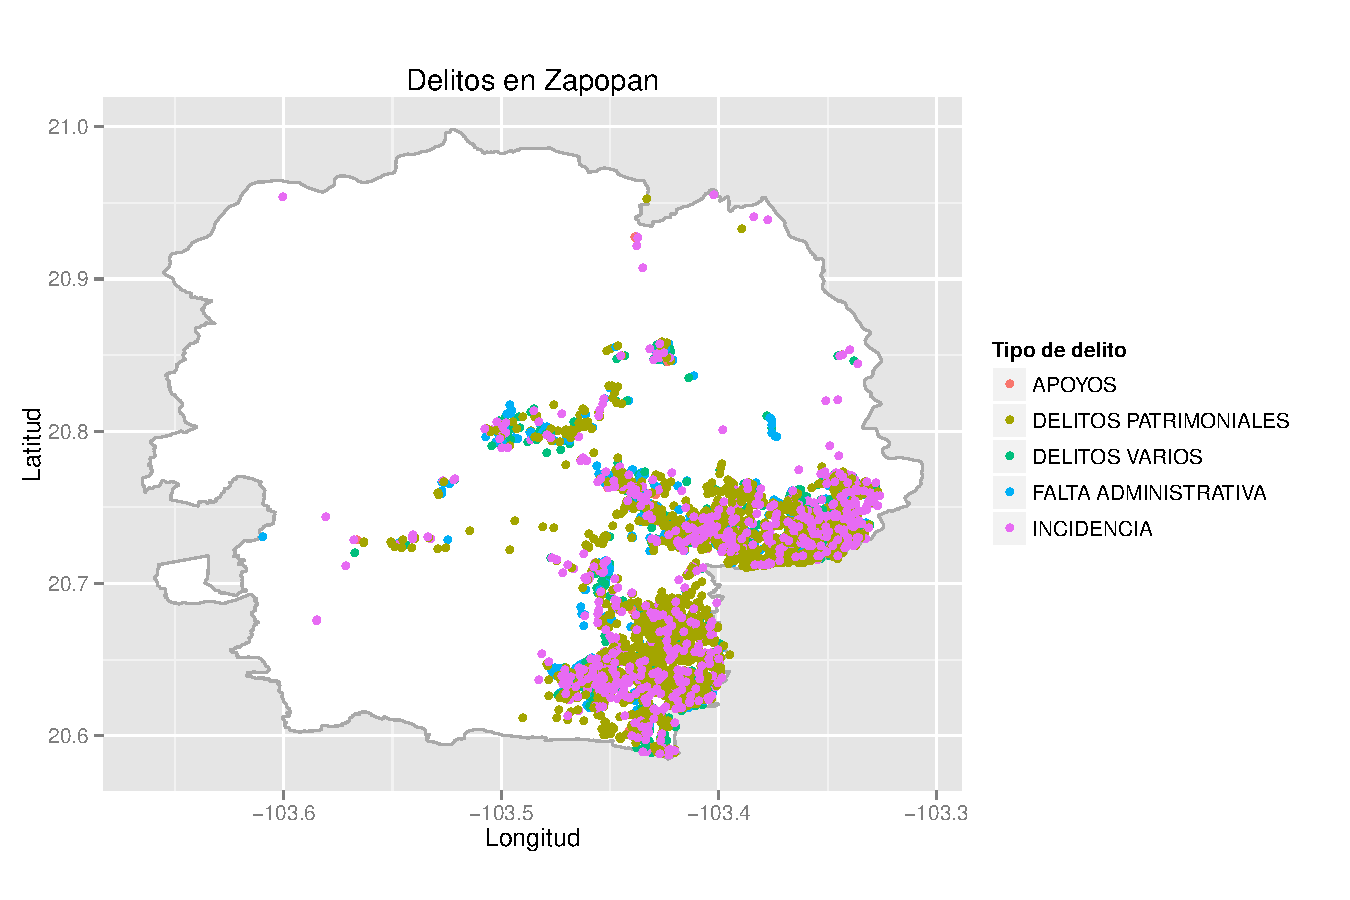
\includegraphics[width=120mm]{../../graphs/zapopan_delitos.pdf}
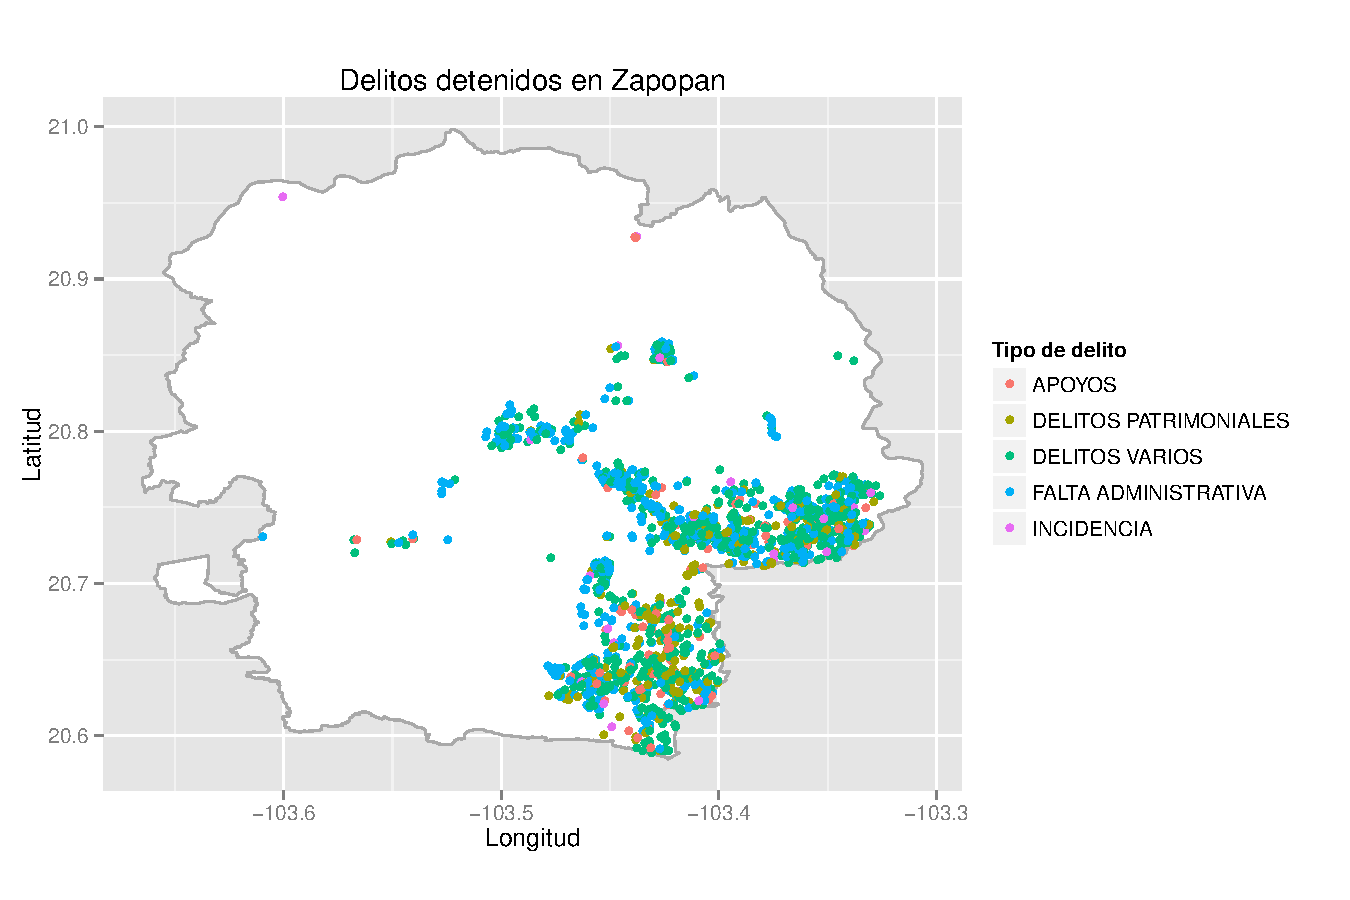
\includegraphics[width=120mm]{../../graphs/zapopan_delitos_detenidos.pdf}
\end{figure}


\begin{table}[h]
\centering
\caption{Número de delitos cometidos y detenidos} 
\begin{tabular}{lrr}
  \hline
Tipo de delito & Cometidos & Detenidos \\ 
  \hline
APOYOS & 101 & 131 \\ 
  DELITOS PATRIMONIALES & 2293 & 398 \\ 
  DELITOS VARIOS & 896 & 1158 \\ 
  FALTA ADMINISTRATIVA & 807 & 3215 \\ 
  INCIDENCIA & 789 &  29 \\ 
   \hline
\end{tabular}
\end{table}

\begin{table}[ht]
\centering
\caption{Porcentaje de delitos cometidos y detenidos} 
\begin{tabular}{lrr}
  \hline
Tipo de delito & \% de cometidos & \% de detenidos \\ 
  \hline
APOYOS & 2 & 3 \\ 
  DELITOS PATRIMONIALES & 47 & 8 \\ 
  DELITOS VARIOS & 18 & 23 \\ 
  FALTA ADMINISTRATIVA & 17 & 65 \\ 
  INCIDENCIA & 16 & 1 \\ 
   \hline
\end{tabular}

\end{table}
